% Ist-Architektur.tex
\section{Ist-Architektur}

\subsection{Ergebnis des Workshops zur Ist-Architektur}

\subsubsection{Positives und Erhaltenwertes}
Als positiv wurde hervorgehoben, dass die aktuelle Architektur, zumindest soweit bekannt, nicht unlösbaren Problemen leidet. 
Das war vor einer Neuimplementierung des FreeDesign-Editor der Fall gewesen. 
Auch Anforderungsänderung und Erweiterungen konnten bisher problemlos umgesetzt werden. 

Die Nutzung von Redux als zentrale Zustandverwaltung, sowie die Anbindung and die Einbindung über \textit{Container}-Objekte wurde positiv geweitet. 

Als undbedingt erhaltenwerte wurde auch die strikte Trennung zwischen Produktdarstellung und Designdarstellung, sowie den grafischen Komponenten zum bearbeiten des Designs bewertet. 

Die grundlegende Strukturierung des Quelltextes innerhalb der Ordner hat ebenfalls bewährt und scheint den Einstieg in das Projekt zu fördern. 

\subsubsection{Schwächen und Probleme}

\subsection{Aspekte der Ist-Architektur}



\subsubsection{Komponenten}
Zunächst wurde als wichtig befunden, aufzuschlüsseln aus welchen fachlichen Hauptkomponenten die Anwendung besteht und wie diese mit einander interagieren.

\subsubsection{Struktur des Quelltextes}
Der Quelltext wurde nach Strukturen untersucht und wie sich Hauptkomponenten innerhalb der Struktur wiederfinden

\subsubsection{Verletzungen der Ist-Architektur }

	
\subsection{Analyse-Werkzeuge}


\subsection{Komponenten des FreeDesign-Editors}

\subsubsection{Externe Schnittstellen}
Der FreeDesign-Editor kommuniziert über folgende vier Schnittstellen:
\begin{itemize}
	\item Über eine grafische Oberfläche wird der Editor vom Nutzer bedient und die Anwendung reagiert sowohl auf Mauseingaben als auch auf Tastatureingaben. 
	\item Zur Kommunikation mit Unitedprint-Backend wird eine REST-API genutzt. 
	\item Der Editor wird mit einer Reihen von URL-Parametern aufgerufen, die steuern, welche Produkt-Konfiguration von der Anwendung geladen wird. Über die URL-Parameter kann auch das Laden von Designvorlagen oder Kundendesign gesteuert, sowie weiter Funktionalitäten des Editors aktiviert werden. 
	Innerhalb des Editor besteht auch die Möglichkeit das Produkt zu ändern, worauf hin die URL sich aktualisiert.
	\item Ein Browser-Cookie wird vorwiegend zur Nutzer-Authentifizierung genutzt. 
\end{itemize}

Browser bieten die Möglichkeiten Daten in einem Local-Storage-Object oder einem Session-Storage-Object Daten zu speichern. \cite{Mozilla:Storage}
Die werden jedoch aktuell von der Anwendung nicht genutzt. 

% TODO: Es fehlt das Clipboard

\begin{figure}[H]
  \centering
  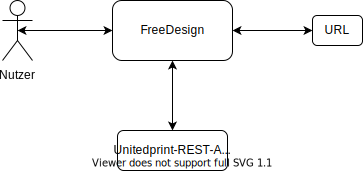
\includegraphics{diagrams/Ist-Architektur/Freedesign_Interaktion.pdf}
   \caption{Externe Schnittstellen}
   \label{fig:Externe_Schnittstellen}
\end{figure}


\subsubsection{Grafische-Oberfläche}

\subsubsection{Anwendung-Zustand}

\subsubsection{Produktkonfiguration}

\subsubsection{Design-Modell}

\subsubsection{Nutzerdaten}

\subsubsection{REST-API-Anbindung}

\subsubsection{Kommandozeilenprogramme}

\subsection{Ordnerstruktur}

\subsubsection{Übersicht der obersten Ordnerstruktur}
Der Quelltextdateien, welche die Anwendungen beschreibt, sind innerhalb des Ordner \emph{src} organisiert. 
% Die obersten Ordnerebene des \emph{src}-Ordner spiegelt die Architektur der Anwendung auf höchster Ebene wider. 
Mit Hilfe des Analysewerkzeug \emph{Dependency cruiser} wurde Abbildung \ref{fig:obersteOrdnerebene}  erstellt, welche eine Übersicht der obersten Ordnerebene gibt, sowie einen Überblick der Zugriffe zwischen den Ordnern. Wird innerhalb eines Ordners Quelltext aus einem benachbarten Ordner importiert, wird dies durch eine Pfeilspitze am benachbarten Ordner gekennzeichnet. 

\begin{figure}[H]
	\centering
    \caption{Eine Übersicht der obersten Ordnerebene, sowie ein Überblick der Zugriffe zwischen den Ordnern.}
	\label{fig:obersteOrdnerebene}
	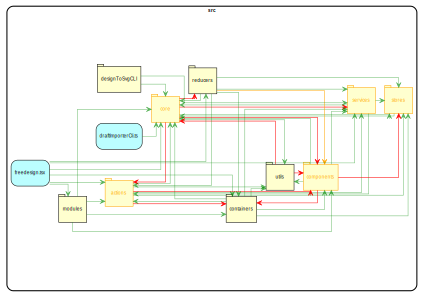
\includegraphics{diagrams/Ist-Architektur/Projektuebersicht.pdf}
\end{figure}

\paragraph{Ordnerinhalte}
Der \emph{core}-Ordner ist für den Anwendungskern vorgesehen und er sollte von der umgebenden Anwendung genutzt, nicht jedoch auf sie zugreifen. Er enthält Geschäftslogik sowie grundlegende Funktionalitäten und Datenstrukturen der Anwendung, die nicht direkt mit \emph{ReactJS} und \emph{Redux} im Zusammenhang stehen. Dem Ordner mangelt es an einer klaren Strukturierung, auf Grund dessen die das richtig Zuordnung und Auffinden der Geschäftslogik schwierig ist. Es kann angenommen werden, dass dies auch einer der Hauptgründe dafür ist, dass Teile der Geschäftslogik aussehrhalb des Anwendungskerns implementiert wurden. 

Sämtlich Komponenten die zur Erzeugung der grafischen Oberfläche genutzt werden, sind innherhalb des Ordners \emph{components} organisiert. Darunter zählen Komponenten zur Erzeugung von Menüs, Dialogen oder auch Werkzeuge zu Designbearbeitung. Alle Komponenten sind unter der Verwendung von \emph{ReactJS} realisiert.

Die Ordner, \emph{reducers}, \emph{action} und \emph{stores}, in dem alle \emph{Redux-States} hinterlegt sind, beziehen sich auf die Verwendung auf von \emph{Redux}. 

Der Ordner \emph{containers} enthält Komponenten, welche die \emph{ReactJS}-Komponenten aus dem Ordner \emph{components} mit den \emph{Redux-State} sowie \emph{Redux-Actions} verbindet. 
Dadurch sind die \emph{ReactJS}-Komponenten nicht an den globalen Zustand der Anwendung gebunden und können mehrfach eingesetzt werden. Ein Beispiel hierfür ist der \emph{Container LoginDialog}, welcher das Anmeldeformular für den Kundenanmeldung erzeugt. Dieser nutzt Formularelemente und Schaltflächen aus dem \emph{components}-Ordner zur Erzeugung der grafischen Oberfläche. Für die Prüfung, ob der Kunden erfolgreich angemeldet ist, greift der Dialog auf die Kundendaten zu, die im \emph{Redux-State} verwaltet werden. Über eine \emph{Redux-Action} wird die Anmeldung durchgeführt, welche vom \emph{Container} aufgerufen wird. Dadurch das die Formularelement und Schaltflächen nicht an den Anwendungszustand gebunden sind, können sie z.B. auch in einem Dialog zur Kundenregistrierung Verwendung finden.

Für die Kommunikation mit der API von Unitedprint wird das Modul \emph{redux-axios-middleware} eingesetzt. 
Das Module ist eine \emph{Redux}-Middleware für die asynchrone HTTP-Kommunikation. HTTP-Anfragen werden durch den Aufruf von \emph{Redux-Actions} ausgelöst, ebenso werden \emph{Redux-Actions} nach eintreffender Antwort ausgelöst \autocite[vgl.][]{ReduxAxios}. Im Ordner \emph{services} sind die \emph{Redux-Actions} für die API-Aufrufe definiert. Desweiteren enthält der Ordner noch eine Serviceklasse zur Kommunikation mit Zwischenablage des Betriebssystems. Die Klasse ermöglicht das einfügen von Text aus der Zwischenablage in das Design, sowie das Kopier von Text aus dem Design in die Zwischenablage.

Im Ordner \emph{utils} befinden sich nur zwei Komponenten, die direkt mit der Browser-API kommunizieren und sich nur innerhalb des Browser aufrufen lassen. Wie bereits im Architektur-Workshop festgestellt, ist die Existenz dieses Ordners fragwürdig uns er sollte aufgelöst werden.

Ebenso zu hinterfragen ist die Existenz des Ordners \emph{modules}. Sein Inhalt könnte auch in den Ordnern \emph{containers} und  \emph{components} untergebracht werden. Es werden innerhalb des Ordners zwei alternative Aufrufe des FreeDesign-Editors realisiert, zum einen der Aufruf für den \emph{Easyprint}-Webshop und zum anderen der Aufruf aus einer internen Anwendung zur Adminstration. Der interne Aufruf unterscheidet sich durch ein Anmeldeformular, welches dem Editor vorgeschallten ist, über welches sich ein Mitarbeiter autorisiert. Somit kann eine Mitarbeiter Zugriff auf ein Kundendesign erlangen und Serviceanfragen bearbeiten. 

Innerhalb des Ordners \emph{styles} sind globale \emph{CSS}-Definition untergebracht, die das optische Erscheinungsbild der Anwendung beschreiben. Die Definitionen werden ausschließlich Komponenten im Ordner \emph{components} verwendete. 


Die Datei \emph{freedesign.tsx} ist die Startdatei des FreeDesign-Editors, über die das Programm betreten wird. Für das Kommandozeilen-Programm \emph{Draft-Importer}, zum Import der Designvorlagen, ist die Datei \emph{draftImporterCli.ts} als Startdatei vorgesehen. Im Ordner \emph{designToSvgCLI}-Ordner wurde ein weiteres Kommandozeilen-Programm implementiert, welches ebenfalls für den Import der Designvorlagen benötigt wird.


\paragraph{Zugriffe}
Die grünen Zugriffspfeile stellen erwartete Zugriffe dar und sind somit gewollte Kopplungen der Einzellkomponenten. Im Gegensatz dazu sind die roten und orangen Zugriffspfeile ungewollte Zugriffe und wurden mit der Zeit integriert. Bei den roten Zugriffen besteht außerdem das Problem, dass diese Zyklen erzeugen und damit gegen die Forderung an eine Architektur, zyklusfrei zu sein, verstoßen. Zyklen schaffen eine gegenseitige Abhängigkeit zwischen den Komponenten und schränken damit die Erweiterbarkeit, Testbarkeit und Verständlichkeit der Komponenten ein \autocite[vgl.][88 - 90]{Lilienthal2019}. 
Es bestehe sowohl einzelne Zyklen, wie zwischen den Ordner \emph{core} und \emph{services} sowie Zyklengruppen. Ein Beispiel hierfür ist die Gruppe bestehend aus \emph{actions}, \emph{utils} und \emph{core}.
Auch innerhalb der Ordner bestehe Zyklen wischen Unterkomponenten. 
Insgerammt wurden 14 Zyklen festgestellt.

% \paragraph{Verwaister Quelltext}
% Innerhalb der orange gekennzeichneten Ordner befinden sich verwaiste Quelltextabschnitte, welche nicht aufgerufen werden. Solche Quelltextstellen können die Verständlichkeit des Quelltext einschänken. 

\paragraph{Kritik}
Eine gute Architektur zeichnet sich, basierend auf Robert C. Martin (\citeyear[S. 196 - 197]{Martin2018}), dadurch aus, dass sie keine Vorgaben über die verwendete Technologien macht und offen gebgenüber Technologieänderungen ist. 
Diese wird von der aktuellen Architektur auf der obersten Ordnerebene nicht erfüllt. Würde z.B. ein Technologwechsel zur Verwaltung des Anwendungszustands durchgeführt werden, würde das einen Änderung der Architektur bedeuten.

Der aktuellen Architektur wurde zum Zeitpunkt ihrer Entwicklung kein Architekturmuster zugrunde gelegt, was viel Raum zu Interpretation der Architektur lässt. 

% \begin{figure}[H]
% 	\centering
% 	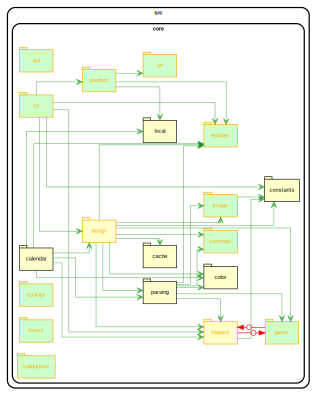
\includegraphics{diagrams/Ist-Architektur/core-graph.pdf}
% 	\caption{Übersicht  }
% 	\label{fig:coreGraph}
% \end{figure}



